% !TeX spellcheck = fr_FR
\begin{resume}

Le \textit{big data} a remis en évidence plusieurs défis pour les systèmes distribués, notamment les fameux "\textit{big V's}" : volume, variété, vitesse. Alors que le volume de données est plus ou moins simple d'être géré et que la vitesse dépend à la fois des ressources et des algorithmes, la variété des données est devenue l'un des points clé dans l'intégration des systèmes d'information\footnote{{\scriptsize \url{http://sloanreview.mit.edu/article/variety-not-volume-is-driving-big-data-initiatives/}}}. S'attaquer à cette hétérogénéité des données devient de plus en plus un défi pour le développement d'applications. 

Sans avoir l'ambition de proposer des solutions nouvelles pour la gestion de la variété de données, ce chapitre présente nos efforts visant à spécifier une plateforme documentaire garantissant un accès transparent à différentes sources d'information, indépendamment de la nature des données (fichiers, flux, bases de données, etc.). Cette spécification repose sur un ensemble d'éléments dédiés à l'indexation, à la recherche et à l'accès aux données. Également, la spécification s'occupe des mécanismes d'interconnexion et de coordination entre les éléments de la plateforme. Grâce à une organisation hiérarchique, cette plateforme a l'avantage de pouvoir être déployée sur une grande variété d'infrastructures.  

La majorité des travaux présentés dans cette partie résultent du travail de thèse de Thierno Ahmadou Diallo, effectuée sous la co-direction de Olivier Flauzac (Université de Reims Champagne Ardenne), de Samba Ndiaye (Université Cheikh Anta Diop, Sénégal) et moi-même. Ces travaux on fait l'objet de publication de deux journaux (\cite{Steffenel2015-Grappes,Steffenel12f}) et quatre conférences (\cite{Steffenel2014-CARI,Steffenel13a,Steffenel13c,Steffenel12d}).



\end{resume}

\section{Introduction}

La gestion de données à grande échelle est un problème récurrent autant dans les domaines scientifiques que dans le monde de l'entreprise. Malgré les constantes avancées en matière de capacité des mémoires et disques, l'utilisation d'un seul dispositif de stockage n'est plus une option vu que l'accès concurrent, la fiabilité, la consommation énergétique et le coût sont des obstacles au développement des systèmes. C'est pour cette raison que les chercheurs et développeurs se sont tournés depuis longtemps vers le développement de solutions de stockage distribué, afin de contourner ces limitations.

Dans les cas où les données peuvent être représentés sous la forme de fichiers, les solutions de type NAS/SAN, réseaux P2P et aussi le stockage dans des infrastructures de type (\textit{clouds}) représentent des choix technologiques capables d'offrir un stockage à grande échelle pour un coût raisonnable. Ces choix concernent aussi les bases de données de type relationnelle ou NoSQL, mais dans ce cas l'accès aux données requiert toujours une entité (pseudo)centralisée capable d'agréger et de présenter les données (ce qui n'exclut pas le traitement parallèle des requêtes). 

À travers différentes stratégies, ces solutions distribuées proposent des solutions transparentes à l'augmentation des besoins de stockage, tout en offrant suffisamment de garanties pour assurer la consistance et la pérennité des données. Aujourd'hui, l'utilisation de solutions de stockage de fichiers sur un NAS/SAN ou sur le \textit{cloud} est devenue aussi courante que l'utilisation de disques ou clés USB, une fois que les ressources potentiellement illimités offerts par les réseaux P2P ou les infrastructures de type \textit{cloud} présentent plusieurs avantages en ce qui concerne le coût, la disponibilité et l'utilisation des ressources physiques. Cependant, ces solutions peuvent aussi présenter des inconvénients liés à la vitesse d'accès et à la sécurité des données ; la solution à ces inconvénients est encore loin d'être garantie et dépend majoritairement des solutions propriétaires proposées par les fournisseurs des services de stockage. Un autre aspect à considérer est la compatibilité entre les systèmes : si certaines APIs rendent la manipulation des fichiers relativement simple, l'intégration d'autres représentations de données est moins évidente. Nous considérons qu'un système de gestion de données doit être capable aussi d'accéder à des requêtes sur une base de données, des flux de données ou encore faire appel à des Web services, le tout d'une manière uniforme et transparente pour l'utilisateur.

C'est dans le but de proposer une architecture unifiée pour les données et les services que nous avons présenté la spécification de la plateforme GRAPP\&S (\textit{GRid Applications and Services}), une architecture générique pour l'agrégation de données et services. Ce framework a été conçu de manière à intégrer de manière transparente les données de type fichier mais aussi les bases de données, les flux (audio, vidéo, données de capteurs et de l'Internet des Objets), les services Web et le calcul distribué. À travers une structuration hiérarchique basée autour du concept de "communautés", GRAPP\&S rend possible l'intégration de sources de d'information disposant de protocoles d'accès hétérogènes et des règles de sécurité variés.

\section{L'Architecture GRAPP\&S \label{SEC:GRAPPES}}

\subsection{Définitions\label{sec:Definitions}}
Pour la définition de l'architecture GRAPP\&S nous considérons un modèle de communication représenté par un  graphe non orienté  et connexe $G = (V, E)$, où $V$  désigne  l'ensemble  des  n{\oe}uds  du système et $E$ désigne l'ensemble des liens de communications qui existent entre les n{\oe}uds. Le modèle utilisé pour notre système est étudié dans \cite{Chalopin06}. Deux n{\oe}uds $u$ et $v$ sont dits adjacents ou voisins si et seulement si ${u, v}$ est un lien de communication de $G$. ${u_i, v_j} \in E$ est un canal bidirectionnel connecté au port $i$ pour $u$ et au port $j$ pour $v$. Donc les n{\oe}uds $u$ et $v$ peuvent mutuellement envoyer ou recevoir des messages en mode asynchrone. 

Un message $m$ en transit est noté $m(id(u), m', id(v))$ où  $id(u)$  est  l'identifiant du n{\oe}ud qui envoie le message, $id(v)$ est  l'identifiant du n{\oe}ud de réception, $m'$ indique le contenu du message. Chaque n{\oe}ud $u$ du système a un identifiant unique $id$ et  dispose de deux primitives : \texttt{send(message)} et \texttt{receive(message)}. Par soucis de clarté, nous introduisons quelques définitions.

%\newdef{definition}{Definition}
\begin{definition}Un n{\oe}ud  est  défini  comme  étant une  capacité de calcul, de stockage, avec  des moyens et des canaux de communications.\end{definition}

\begin{definition}Une donnée  brute  est  un flux  d'octets qui peut être  sous  différentes formes : une base de données objets ou  relationnelle, un fichier (texte et hypertexte, XML), un flux (vidéo, audio, VoIP),  des  requêtes  de  base  de données ou des résultats issus d'un calcul/service.\end{definition}

\subsection{Communication et les Réseaux \textit{Overlay}}
Le modèle de communication présenté en Section \ref{sec:Definitions} est suffisamment générique pour ne pas inférer sur la manière dont les messages sont effectivement livrés, se limitant uniquement à la définition des propriétés de communication bidirectionnelles entre deux vertex. Pour cette raison, l'architecture de GRAPP\&S peut s'appuyer sur n'importe quel un réseau de communication \textit{overlay} qui garantit une communication bidirectionnelle fiable et qui permet d'explorer différents chemins de communication pour chaque arête dirigée (réseau routé). Ceci donne une plus grande liberté d'implémentation et d'adaptation à l'environnement d'exécution, vu que les opérations send/receive peuvent être implémentées de différentes façons, selon les capacités de communication des n{\oe}uds. Dans ce cas, trois scénarios principaux peuvent être considérés : 
\begin{itemize}
	\item \texttt{Push}, où l'émetteur est capable d'envoyer un message directement au destinataire ;
	\item\texttt{Pull}, où le récepteur cherche régulièrement des messages en attente (ce modèle est fréquemment utilisé dans le cas des réseaux derrière un NAT/pare-feu) ; et 
	\item\texttt{Proxy}, où les voisins doivent passer par un n{\oe}ud intermédiaire afin d'échanger des messages (par exemple, grâce à un \textit{middleware} \textit{publisher/subscriber}). 
\end{itemize}
Dans ces trois scénarios, il est toujours possible d'établir un voisinage direct ou partiel entre les processus, ce qui est compatible avec le modèle par graphes connectes dirigés et qui répond donc aux besoins de l'architecture GRAPP\&S. 


\subsection{Éléments de l'Architecture GRAPP\&S}

Afin de présenter notre architecture, nous introduisons dans un premier temps quelques notations. Une communauté ($C_i$) est une entité autonome, qui regroupe des n{\oe}uds qui peuvent se communiquer et qui partagent une propriété définie : même localisation, même autorité d'administration (des serveurs distants appartenant à la même entreprise, par exemple) ou même domaine d'application (base de données métier, par exemple). Une communauté contient un seul processus \textit{Communicator} ($c$) et au moins un processus \textit{Ressource Manager} ($RM$) et un \textit{Data Manager} ($DM$) et ces processus sont organisés de façon hiérarchique dans une communauté. L'interconnexion entre différentes communautés C se fait grâce à des liens de voisinage point-à-point entre les processus Communicator.

\subsubsection*{Communicator (\textit{c})}
Le n{\oe}ud \textit{Communicator} (\textit{c}) joue un rôle essentiellement lié au transport d'informations et à l'interconnexion entre différentes communautés, comme par exemple lors du passage de messages à travers des pare-feu. C'est le point d'entrée de la communauté, et il assure sa sécurité vis-à-vis de l'extérieur, grâce à l'établissement de \textit{Service-Level Agreements} (SLAs) avec les autres communautés. De même, le communicateur coordonne la sécurité intérieure de la communauté, et peut modifier ses politiques d'accès grâce à des décisions prises au sein de la communauté \cite{Steffenel12a}. Un n{\oe}ud \textit{c} dispose d'un identifiant unique (ID) à partir duquel on construit les identités des autres n{\oe}uds de la communauté. Ce n{\oe}ud ne stocke pas de données et ne fait pas d'indexation.

\subsubsection*{Ressource manager (\textit{RM})} 
Les processus \textit{Ressource Manager (\textit{RM})} assure l'indexation et l'organisation des données et services dans la communauté. Ils reçoivent les requêtes des utilisateurs et assurent leur prétraitement. Les n{\oe}uds \textit{RM} participent à la recherche de données dans la communauté. Pour des fins de tolérance aux fautes et performance, les informations indexées par les \textit{RM} peuvent être redondantes et/ou partiellement distribuées (DHTs, par exemple). Afin de rendre plus performante la coordination des RMs, nous préconisons l'élection d'un RM désigné (voir section \ref{SEC:Community}).

\subsubsection*{Data manager (\textit{DM})} 
Les processus \textit{Data Manager (\textit{DM})} interagissent avec les sources de données, qui peuvent être dans différents supports tels que les bases de données (objet ou relationnelle), les documents (texte/XML/multimédia), des flux (vidéo, audio, VoIP), des données issues de capteurs ou encore une service hébergé dans le \textit{cloud}. 
Un n{\oe}ud DM est un service qui dispose des composants suivants : 
\begin{enumerate}
	\item[\textit{(i)}] une interface (proxy) adaptée aux différentes sources de données (disque dur, serveur WebDAV, FTP, base de données, stockage sur \textit{cloud} type Dropbox, etc.) et reliée à ceux-ci par un protocole de connexion spécifique au type de donnée, par exemple JDBC, ODBC, FTP, etc ;
	\item[\textit{(ii)}] un gestionnaire de requêtes qui permet d'exprimer des requêtes locales ou globales ; et 
	\item[\textit{(iii)}] un gestionnaire de communication qui permet au n{\oe}ud \textit{DM} de communiquer avec le n{\oe}ud \textit{RM} auquel il est connecté. 
\end{enumerate}

\section{Gestion de la Communauté\label{SEC:Community}}

GRAPP\&S peut être déployé dans plusieurs types d'architecture selon le placement des n{\oe}uds. Dans le modèle de placement (\textit{i}), les n{\oe}uds peuvent être regroupés dans une seule machine physique (voir Figure \ref{fig:noeuds}a). C'est l'exemple typique d'une machine d'un particulier, qui souhaite héberger une communauté de l'architecture. Le placement des n{\oe}uds sous cette forme peut être justifié par sa simplicité à mettre en {\oe}uvre lors de sa phase d'implémentation, en utilisant les concepts d'héritage et de polymorphisme. Les n{\oe}uds sont interconnectés par des sockets, des solutions RPC pour qu'ils puissent communiquer par message dans les deux sens entre deux n{\oe}uds. 

\begin{figure}
	\centering
	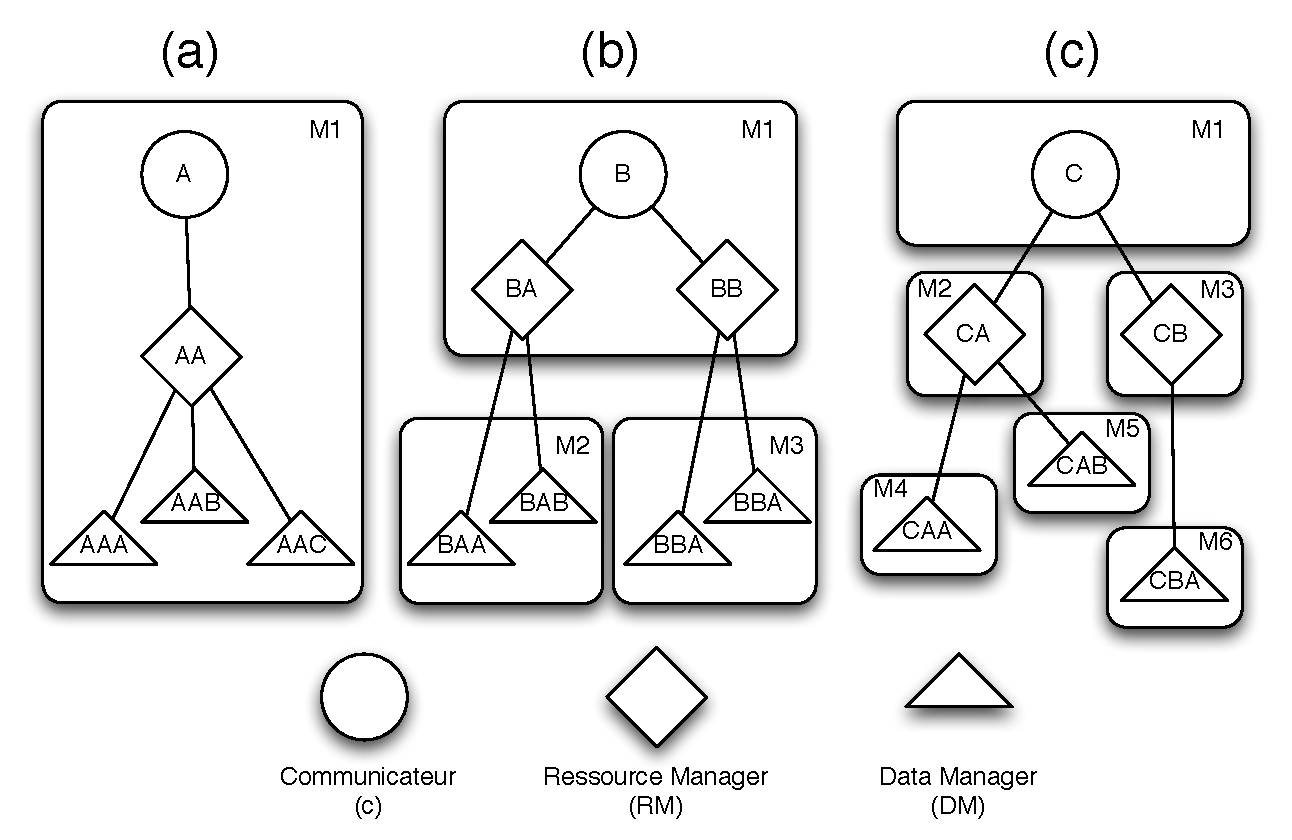
\includegraphics[width=0.85\linewidth]{img/noeuds.pdf} 
	\caption{Organisation des n{\oe}uds (a) dans une machine, (b) dans un \textit{cluster} et (c) dans un réseau\label{fig:noeuds}}
\end{figure}

Dans (\textit{ii}) les n{\oe}uds sont organisés dans une ferme de serveurs telle qu'un \textit{cluster}, ce qui est caractéristique des réseaux HPC (Figure \ref{fig:noeuds}b). Finalement, (\textit{iii}) les n{\oe}uds peuvent être regroupés s'ils partagent une même propriété de localisation ou d'administration (voir Figure \ref{fig:noeuds}c). Ceci est l'exemple d'un réseau formé par les n{\oe}uds d'une entreprise ou d'un laboratoire de recherche. 

Chaque n{\oe}ud de GRAPP\&S a un identifiant (ID) unique. Les adresses IP ou MAC ne sont pas des identifiants suffisamment précis car ils ne permettent pas d'identifier de manière unique les différents n{\oe}uds qui peuvent résider sur une même machine (par exemple, un $RM$ et plusieurs $DM$). De plus, l'utilisation des adresses IP ou MAC ne garantit pas une identité unique, vu que les adresses IP privés peuvent être réutilisées tout autant que les adresses MAC. En effet, l'utilisation massive de la virtualisation commence à poser des problèmes vis-à-vis de la réutilisation des adresses MAC, posant aussi des problèmes au niveau du le déploiement des réseaux IPv6\footnote{\url{http://tools.ietf.org/html/draft-gont-v6ops-slaac-issues-with-duplicate-macs-00}}. Ainsi, nous préconisons l'utilisation d'un mécanisme d'adressage inspiré par JXTA [8]. Dans le cas de GRAPP\&S, chaque n{\oe}ud dispose d'une chaîne unique $ID_{local}$ de 128bits, sous la forme "\texttt{urn:nom\_communaute:uuid:chaine-de-bit}". L'expression de l'adressage hiérarchique se fait par la concaténation des IDs sous forme de préfixe, c'est à dire., l'ID du n{\oe}ud $c_i$ est équivalent à son $ID_{local}$, l'ID du n{\oe}ud $RM_i$ est formé par $ID_{c_i}/ID_{RM_i}$, et l'ID du n{\oe}ud $DM_i$ présente la forme $ID_{c_i}/ID_{RM_i}/ID_{DM_i}$.

Un avantage de l'utilisation d'un modèle d'adressage propre à GRAPP\&S est que cela le rend indépendant du modèle d'adressage du réseau \textit{overlay} sur lequel GRAPP\&S est implémenté. Ainsi, deux communautés GRAPP\&S implémentées sur des \textit{middlewares} différents (FreePastry\footnote{\url{http://www.freepastry.org}} et Phex\footnote{\url{http://www.phex.org}}, par exemple) seront toujours compatibles, une fois la connexion établie entre leurs \textit{communicator}. 

\subsection{Gestion des N{\oe}uds}
La topologie du réseau change fréquemment à cause de la mobilité des n{\oe}uds. Nous travaillons dans l'hypothèse où les tout n{\oe}ud qui arrive dans le réseau est initialement un n{\oe}ud DM. Selon les conditions de l'environnement où ce n{\oe}ud se trouve, il peut se voir attribuer des rôles supplémentaires et "monter" dans la hiérarchie.

\subsubsection*{Connexion d'un n{\oe}ud}

Quand un n{\oe}ud $DM$ arrive dans le réseau, il dispose de deux moyens pour trouver un n{\oe}ud $RM$ sur lequel il peut se connecter :
\begin{itemize}
	\item Si le n{\oe}ud $DM_i$ connait un ou plusieurs n{\oe}uds $RM$, il envoie un message de diffusion \texttt{Hello()} et collecte toutes les identités des n{\oe}uds $RM$, qu'il garde dans un tableau ordonné par l'identifiant. Il peut ainsi se connecter au n{\oe}ud \textit{RM} qui a l'identifiant le plus grand. Si ce dernier se déconnecte, alors le $DM_i$ le supprime du tableau et se connecte au n{\oe}ud $RM$ suivant ; 
	\item Si par contre le n{\oe}ud $DM$ ne connait aucun n{\oe}ud $RM$, il doit effectuer une découverte sur le réseau local (par exemple, grâce à un multicast) ou contacter un service d'annuaire qui peut indiquer l'identifiant d'un n{\oe}ud $RM_i$. Comme la manière de trouver le n{\oe}ud $RM_i$ dépend de l'implémentation, elle n'est pas précisée dans notre architecture.
\end{itemize}
Finalement, si aucune tentative de connexion à un n{\oe}ud $RM$ (et par extension, un n{\oe}ud \textit{c}) ne réussit, le n{\oe}ud $DM$ a la possibilité de former sa propre communauté. Il assume ainsi les trois rôles $c$, $RM$ et $DM$, jusqu'à ce que d'autres n{\oe}uds le rejoignent. À ce moment, une élection pourra avoir lieu afin de redistribuer les rôles entre les n{\oe}uds.

\subsubsection*{Déconnexion d'un n{\oe}ud} 

Les n{\oe}uds peuvent subir des déconnexions volontaires ou involontaires (pannes). Comme le cas des déconnexions volontaires est trivial, nous nous concentrons ici sur les déconnexions involontaires.

Entre deux niveaux hiérarchiques, les pannes peuvent être détectées soit par des messages périodiques de type \textit{Pull} (aussi connu comme \textit{heartbeat}), à la demande par des messages \textit{Push} (\textit{ping-pong}) \cite{Chandra96} ou encore en s'appuyant sur un mécanisme propre au \textit{middleware} \textit{overlay}. Pour les n{\oe}uds appartenant à un même niveau hiérarchique, la surveillance peut aussi se faire grâce à un mécanisme de passage de jetons "de service". Cela permet non seulement l'allégement du mécanisme de détection (il suffit de surveiller son prédécesseur et son successeur) comme permet la diffusion rapide des informations à l'ensemble des n{\oe}uds.

Pour la mise en place d'un mécanisme générique de détection de défaillances, nous préconisons une procédure en deux étapes. 
Tout d'abord, chaque n{\oe}ud dispose d'une liste de voisins \{$N_1,…,N_n$\} composée des n{\oe}uds en contact direct (par exemple, un $RM_i$ est en contact avec son $c$, ses $DMs$ et ses voisins $RM_{i-1}$ et $RM_{i+1}$. À cette liste de voisins est associé une liste de temporisateurs d'attente \{$ta_1,…,ta_n$\}. 

Lorsque aucun message du n{\oe}ud $N_k$ n'est reçu jusqu'à l'expiration du temps $ta_k$, une suspicion de défaillance est levée et doit être vérifiée auprès d'un deuxième n{\oe}ud qui est aussi en contact direct avec le n{\oe}ud suspect. Ainsi, si la suspicion concerne le n{\oe}ud $c$, un n{\oe}ud $RM_i$ interroge son voisin direct $RM_{i+1}$ avec un message jeton initialisé à \texttt{faux}. Si $RM_{i+1}$ a reçu un message du n{\oe}ud $c$ avant l'expiration de son temps d'attente $ta_c$, $RM_{i+1}$ modifie la valeur du jeton à \texttt{vrai} et retourne le message jeton à son émetteur $RM_i$. Ceci signifie (indirectement) que le n{\oe}ud $c$ n'est pas déconnecté et le n{\oe}ud $RM_i$ peut envoyer à nouveau un message au n{\oe}ud $c$. Si par contre $RM_{i+1}$ n'a pas été contacté récemment par $c$, il fera suivre un jeton la valeur \texttt{faux} qui, grâce au passage du jeton, alertera tous les n{\oe}uds $RM$ \{$RM_1,…,RM_n$\} de la défaillance de $c$.

De manière similaire, si un n{\oe}ud $c$ suspecte un n{\oe}ud $RM_k$, il peut demander confirmation à $RM_{k+1}$. Évidemment, cette procédure générique peut s'adapter aux différentes situations telles qu'un n{\oe}ud qui contient un $RM$ et plusieurs $DM$. Dans ce cas, le mécanisme de détection peut être allégé pour mieux répondre aux caractéristiques du n{\oe}ud. 

À la suite de la confirmation d'une défaillance, les n{\oe}uds concernés doivent \textit{(i)} mettre à jour leurs informations (liste de voisin, tableaux d'index, etc.) et éventuellement (\textit{ii}) procéder à l'élection d'un nouveau $RM$ (respectivement c) qui prendra en charge les éventuels $DM$ (ou $RM$) orphelins.  

\subsection{Coordination entre les N{\oe}uds}

Vu le caractère dynamique et volatile des réseaux informatiques, il est important de garantir la coordination entre les n{\oe}uds, notamment dans le cas des $RM$. Une manière simple et performante de faire ceci est de définir un n{\oe}ud avec des responsabilités étendues au sein de son groupe, ce choix étant fait par exemple grâce à une élection. 

L'élection d'un n{\oe}ud peut être nécessaire en deux situations : soit pour remplacer un n{\oe}ud défaillant et garantir la continuité du service (par exemple, lors de la panne d'un n{\oe}ud $c$), mais aussi pour simplifier la coordination entre les n{\oe}uds de même type, avec par exemple l'élection d'un $RM$ qui agirait comme "super-node" pour l'indexation de données et services. 

Il faut noter que la connaissance préalable des n{\oe}uds du niveau supérieur n'est pas obligatoire, vu que différentes techniques permettent d'obtenir les identifiants des autres n{\oe}uds. La méthode la plus simple consiste à utiliser directement le mécanisme d'adressage GRAPP\&S : étant indépendant du \textit{middleware} de communications, ce système d'adressage permet facilement de remonter la hiérarchie GRAPP\&S et de contacter d'autres n{\oe}uds (grâce au routage du réseau \textit{overlay}). Il suffit donc de remonter les niveaux de son propre identifiant ou de contacter d'autres n{\oe}uds dont on récolté les identifiants (ceux dont on a reçu des requêtes récemment, par exemple). Cette technique permet aussi de contacter d'autres \textit{communicators} $c_j$ et de réintégrer un réseau de communautés auprès la déconnexion involontaire de son \textit{communicator} $c_i$. En dernier recours, GRAPP\&S peut s'appuyer sur les éventuels mécanismes de découverte de topologie (broadcast/multicast) offerts par le propre \textit{overlay}.

Vu que le problème de la reconnexion au reste de la communauté peut être traité de manière plus ou moins simple au sein de la propre architecture GRAPP\&S, il est intéressant de se pencher sur les algorithmes d'élection eux-mêmes. Dans GRAPP\&S, nous préconisons un algorithme d'élection distribué inspiré des protocoles de routage OSPF et IS-IS \cite{rfc1142,rfc2328,ISISxOSPF}. En effet, les n{\oe}uds GRAPP\&S disposent d'un identifiant unique qui peut être utilisé de manière systématique par ces algorithmes d'élection. 

Le choix entre les algorithmes de IS-IS ou d'OSPF est plus lié aux préférences d'implémentation et à l'hétérogénéité des n{\oe}uds. En effet, l'algorithme d'élection de IS-IS est de type déterministe, où l'élu est toujours le n{\oe}ud avec le plus grand identifiant (appelé \textit{DIS - Designated IS}). Ce mécanisme est simple à implémenter et ne requiert pratiquement aucun échange d'informations car les n{\oe}uds disposent déjà d'une liste avec les identifiants de leurs voisins, il ne resterait que le coût associé à la prise de fonctions d'un n{\oe}ud élu à un rôle différent de celui qu'il occupait précédemment. L'inconvénient de cette technique est qu'un réseau avec un fort taux de volatilité peut occasionner des élections à répétition, soit lors de la déconnexion du leader, soit lors de la connexion d'un n{\oe}ud avec un identifiant prioritaire.

Dans les cas où la volatilité risque d'impacter la performance du réseau, il est possible d'utiliser un mécanisme non-déterministe comme celui d'OSPF \cite{ISISxOSPF}. Dans ce type d'algorithme, plus conservateur, le choix d'un leader (\textit{DR - Designated Router}) n'est nécessaire que si le leader actuellement en place disparaît. Ainsi, l'entrée de nouveaux n{\oe}uds dans la communauté a un impact moins important sur le fonctionnement du réseau.

 \section{Opérations dans GRAPP\&S\label{SEC:OPERATIONS}}

\subsection{Stockage et Indexation}

Le stockage de donnée dans le réseau GrAPP\&S fait intervenir les n{\oe}uds Data Manager $DM$, alors que les n{\oe}uds Ressource Manager $RM$ permettent d'indexer les données et les services. À la fin, chaque donnée est identifiée de manière unique grâce à l'identifiant du n{\oe}ud $DM$, auquel s'ajoute une extension contenant des informations et le type MIME des données. Ceci permet de franchir la barrière du simple "nom de fichier", et peut donc faire cohabiter des données statiques (fichiers), des données dynamiques (requêtes sur une base de données, résultats d'un calcul) et des données à caractère temporaire (flux voix ou vidéo, état d'un capteur, etc.). 

L'ajout d'une nouvelle donnée dans le réseau se fait ainsi : quand un n{\oe}ud $DM_i$ arrive dans le réseau, il se connecte à un n{\oe}ud $RM$ et publie les caractéristiques de ses données pour être indexées. Toute modification des données sur un $DM$ sont propagées au $RM$ auquel il est connecté, qui par la suite peut mettre à jour ces informations et les partager avec les autres $RM$. 

Cette propagation des informations peut prendre différentes formes selon les politiques utilisées lors de l'implémentation du réseau des $RM$. Une implémentation qui veut garder la simplicité pourra simplement garder un index local sur chaque $RM$, qui sera consulté lors d'une recherche. Au contraire, une implémentation souhaitant minimiser les échanges lors d'une recherche de données penchera sur l'utilisation d'un super-n{\oe}ud au sein des $RM$s ou d'un mécanisme de DHT. Il est aussi possible de favoriser la réplication des index et des données, ce qui exige une coordination entre les $RM$ afin de garder la cohérence des copies. Dans tous les cas, la surcharge des fonctionnalités d'un n{\oe}ud ("super-node") n'est pas une obligation dans notre structure mais simplement une spécificité pouvant être présente dans une implémentation donnée. 

\subsection{Recherche}
Quand un client cherche une donnée sur GRAPP\&S, il entre en contact avec un proxy $DM_i$, qui envoie une requête $Y$ contenant des informations qui identifient la donnée ou le service. Cette recherche dans une communauté de GrAPP\&S se fait par paliers, de manière à respecter l'organisation hiérarchique du réseau. La Figure \ref{fig:routage} illustre une partie de cette procédure de recherche : 
\begin{enumerate}
	\item Un n{\oe}ud $DM_i \in C_i$ envoie la requête a son n{\oe}ud $RM_i \in C_i$ ;
	\item $RM_i$ vérifie dans son indexe s'il y a parmi ses voisins un $DM$ qui contient la donnée recherchée ;
	\item Si oui, alors le n{\oe}ud $RM_i$ retourne au n{\oe}ud $DM_i$  une liste de n{\oe}uds $DM$ qui contiennent l'information recherchée ;
	\item Sinon, le n{\oe}ud $RM_i$ fait suivre la requête, soit directement aux voisins $RM_k \in C_i$ (si le mécanisme de communication le permet), soit à son n{\oe}ud $c_i \in C_i$ pour retransmission aux autres $RM_k \in C_i$ ;
	\item Quand un  n{\oe}ud $RM_k \in CM_i$ trouve la bonne réponse, alors la requête sera retournée au n{\oe}ud $DM_i$ émetteur en suivant le chemin inverse ;
	\item Si la donnée recherchée n'est pas dans la communauté $CM_i$, alors le $c_i$ fait suivre la requête vers d'autres communautés $CM_j$.  
\end{enumerate}

\begin{figure}
	\centering
	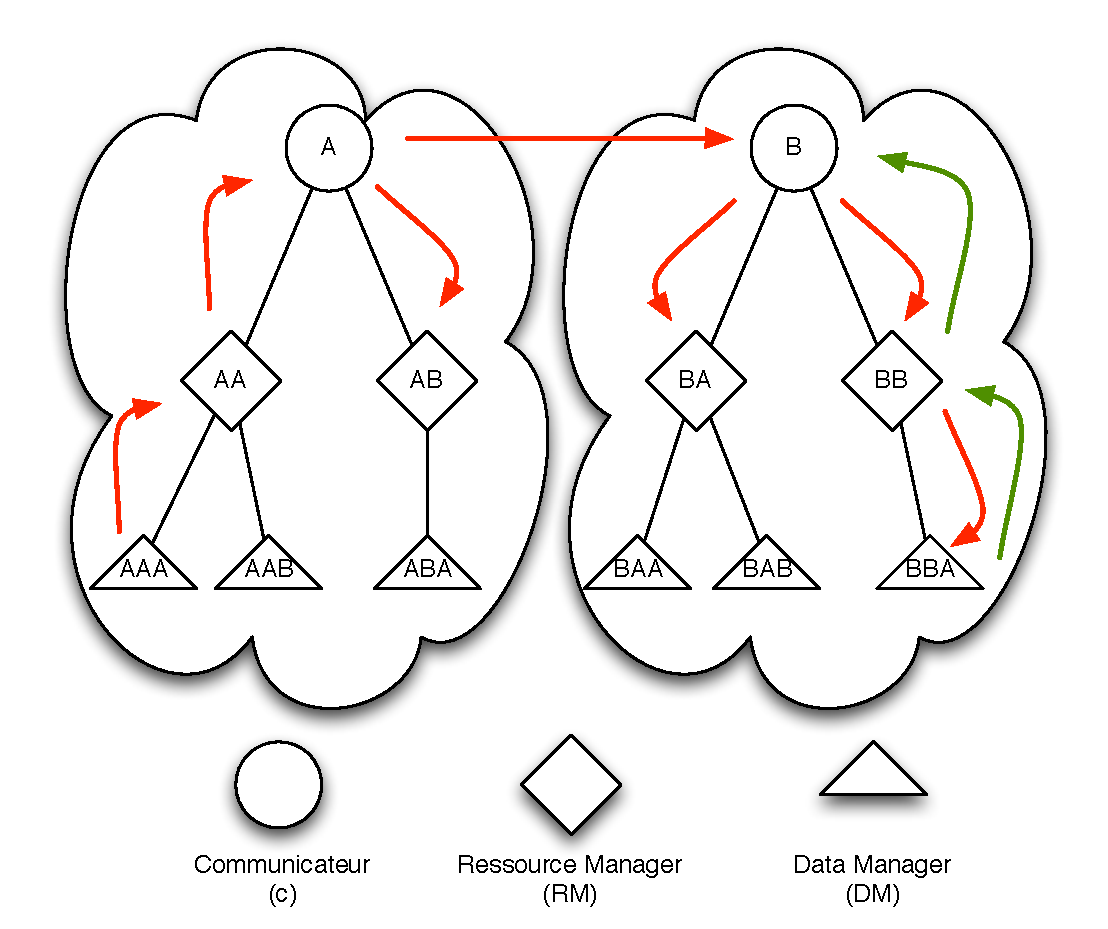
\includegraphics[width=0.8\linewidth]{img/Routage1.pdf} 
	\caption{Recherche d'une information dans GRAPP\&S et mécanisme de routage préfixé\label{fig:routage}}
\end{figure}

En cas de réussite, le client obtient l'identifiant du n{\oe}ud $DM_x$ responsable par la donnée. Dans ce cas, le client a deux possibilités pour accéder à la donnée, soit par connexion directe, soit par une connexion routée. Dans le cas de la connexion directe, le client fait une requête directe au n{\oe}ud $DM_x$ afin d'accéder à la  donnée. Comme le client peut se trouver dans un autre réseau qui ne permet pas l'accès directe à $DM_x$, la connexion peut se faire par routage interne dans GrAPP\&S. Cela se fait de la manière suivante :
\begin{itemize}
	\item Le client, par intermède d'un n{\oe}ud $DM_i$, envoie une requête \texttt{Req($id(DM_x, Y, id(c_i)$)} au n{\oe}ud communicateur $c_i$ ;
	\item  le n{\oe}ud $c_i$, par routage préfixé, envoie la requête \texttt{Req} vers le n{\oe}ud $RM$ qui a indexé la donnée ;
	\item  Ce dernier fait suivre la requête vers le n{\oe}ud $DM_x$ responsable de la donnée ;
	\item Une fois la donnée trouvée, le n{\oe}ud $DM_x$ retourne la bonne réponse au client en suivant le chemin inverse.
\end{itemize}   

Ce mécanisme de recherche hiérarchique empêche l'inondation des liens du réseau. La hiérarchisation permet de définir des chemins par lesquels transitent les requêtes et comme la connectivité logique de notre architecture est par définition de $(n-1)$, il suffit d'appliquer un algorithme de type PIF (\textit{Propagation of Information with Feedback} \cite{Seg83}) pour agréger les requêtes et réduire le nombre de messages d'une recherche.  


\section{Bilan et Perspectives}

Ce chapitre présente une spécification pour une plateforme distribuée basée sur les principes des réseaux hiérarchiques et visant l'établissement d'une base documentaire générique et extensible. Contrairement aux autres travaux que j'ai pu développer autour des systèmes distribués, l'objectif ici n'était pas celui de la distribution de tâches de calcul et leur gestion mais plutôt celui de l'indexation et de la recherche de documents et des sources d'information, le tout afin de minimiser l'hétérogénéité dans l'accès aux données. 

Bien que présente dans la spécification proposée, la coordination des n{\oe}uds fut d'abord conditionnée à la création et à la maintenance de réseaux de proximité pour cette gestion documentaire. La spécification de GRAPP\&S a aussi une qualité moins évidente, celle de l'indépendance vis-à-vis des technologies d'implémentation. De par sa propre organisation en "communautés", différentes instances de GRAPP\&S peuvent s'interconnecter et échanger des données, selon des politiques SLA définies par chaque partie.   

Également, la spécification de GRAPP\&S a permis une meilleure compréhension des différents mécanismes liés à la coordination et gestion des n{\oe}uds dans les réseaux hiérarchiques. En effet, la majorité de mes travaux repose sur une organisation uniforme du réseau où tous les n{\oe}uds possèdent les mêmes prérogatives ou au moins disposent de mécanismes de communication directe entre-eux. Dans le cas d'un réseau hiérarchique, les prérogatives dépendent du rôle joué par les n{\oe}uds, ce qui apporte des défis différents de ceux que je traite habituellement, soit dans le cas des réseaux P2P, soit dans le cas de l'algorithmique distribuée \cite{Steffenel08a,Steffenel09c}. 

Après avoir conclu la spécification de GRAPP\&S, les travaux de thèse de M Diallo se sont tournés vers la recherche et la description de scénarios d'applications, comme par exemple dans le cas de l'\textit{e-learning}. Malheureusement, cela s'est fait au détriment de l'implémentation d'un prototype.  Certains concepts développés restent néanmoins présents dans les autres travaux que je développe, comme par exemple le concept de communautés.  D'une autre part, je développe des activités d'enseignement autour du \textit{big data} qui me permettent d'être en contact direct avec les nouvelles technologies dans ce domaine.